\section{Zašto je nastala SSD mreža}
\emph{Single Shot MultiBox Detector} (dalje \emph{SSD}) je mreža za detekciju i klasifikaciju kojoj je primarna svrha jednostavnost i brzina.
Prije nastanka \emph{SSD} mreže, najpoznatije mreže za isti zadatak bile su implementirane arhitekturom \emph{Region-Convolutional Neural Network} (dalje \emph{R-CNN}).
\emph{R-CNN} mreže na izlazu tipično daju set kvadrata koje opisuju objekt i klasu istog.
Klasični izlaz iz \emph{R-CNN} mreže vidljiv je na slici ~\ref{fig:ObjectDetectionOutput}.
Osim bazičnog, iz \emph{R-CNN}-a nastale su i mreže \emph{Fast(er)-R-CNN} koje dalje ubrzavaju i poboljšavaju preciznost iste arhitekture (\cite{ren2015faster}).
No, nijedna od tih nije uspjela doseći gotovo "real-time" brzinu sa značajnom preciznosču
\begin{figure}[h!]
	\centering
	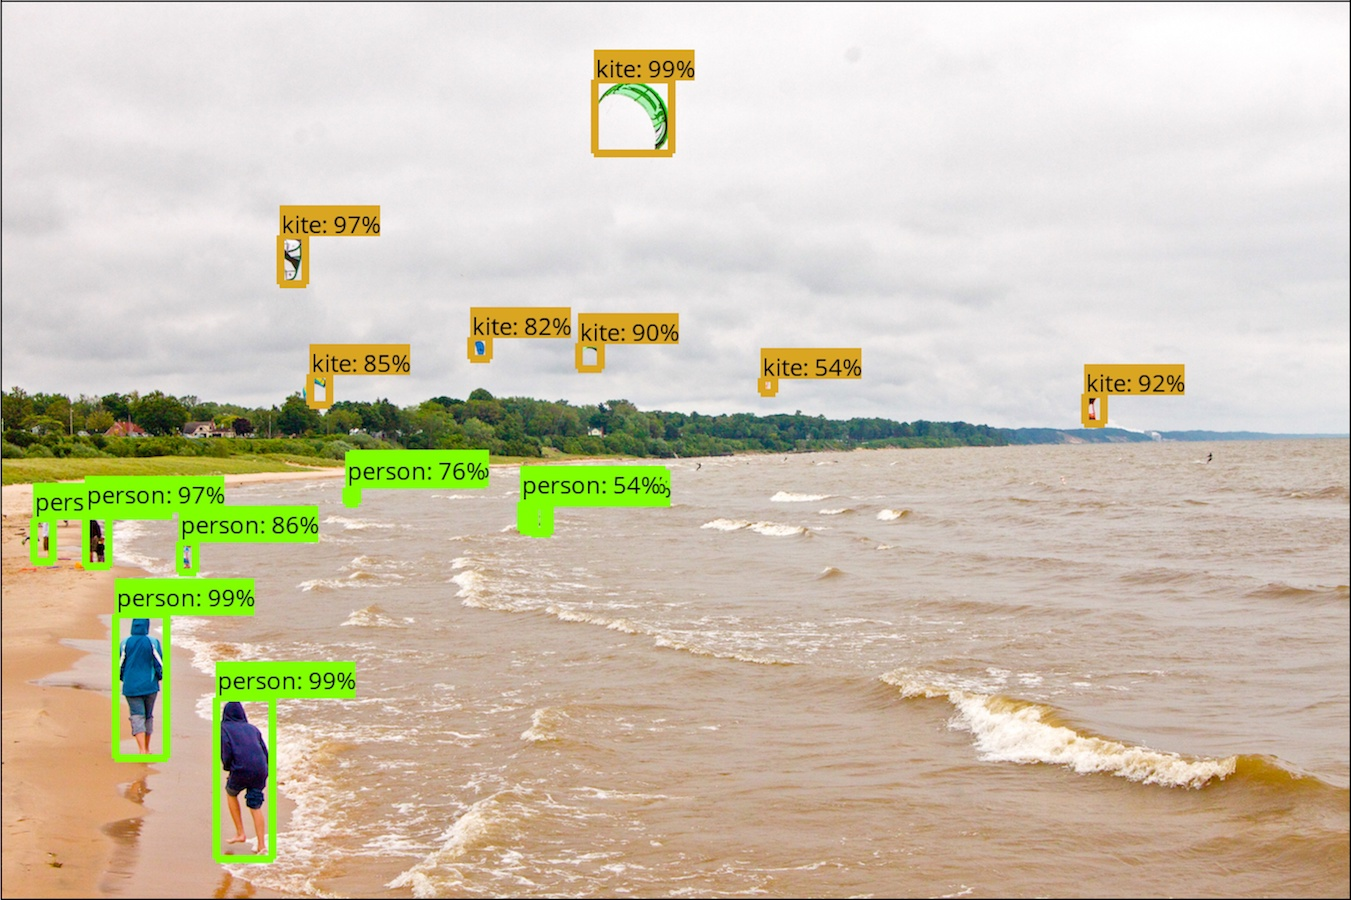
\includegraphics[width=1.0\linewidth]{object_detection_output}
	 \caption{Tipični izlaz iz mreže za detekciju i klasifikaciju sa prikazanim kvadratima i klasama}
 	 \label{fig:ObjectDetectionOutput}
\end{figure} \\
Iako su spomenute mreže imale pokazivale impresivne rezultate, također su imale i nekolicinu problema:
\begin{itemize}
\item Više faza treniranja
\item Komplicirana mreža
\item Mreža spora za stvarno korištenje
\end{itemize}
Zbog spomenutih problema, nastale su nove arhitekture od kojih je jedna i \emph{SSD}, koju ovaj rad koristi cjelokupnu implementaciju zadatka detekcije i klasifikacije 14 različitih klasa.

\section{Arhitektura}
\subsection{VGG-16 arhitektura}
\emph{VGG-16} je poznata neuronska mreža nastala na Oxfordu od strane \emph{Visual Geometry Group}-a, odakle i potječe ime.
Mreža sama po sebi ostvaruje odlične rezultate na \emph{ImageNet} datasetu no to nije jedini razlog zašto je jedna od najkorištenijih. \\
\emph{VGG} mreža razvijena je da bude jednostavna, sadržavajući samo \texttt{3x3} konvolucijske i \texttt{2x2} pooling slojeve prije završnih gusto spojenih slojeva (\cite{simonyan2014very}).
Arhitektura mreže vidljiva je na slici ~\ref{fig:VGGArchitecture}
Također, cijela struktura, težine i cijela istrenirana mreža je dostupna besplatno na internetu na službenoj stranici projekta (\url{http://www.robots.ox.ac.uk/~vgg/research/very_deep/}).
\begin{figure}[h!]
	\centering
	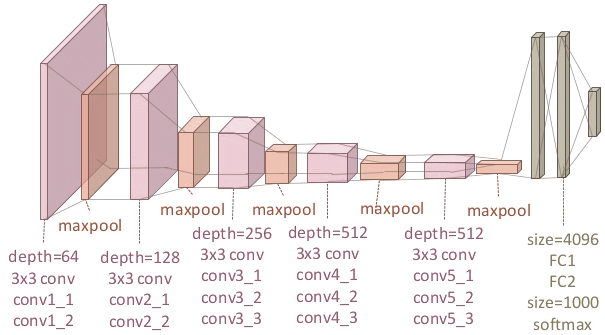
\includegraphics[width=1.0\linewidth]{vgg_architecture}
	 \caption{Arhitektura VGG-16 mreže}
 	 \label{fig:VGGArchitecture}
\end{figure}
Mana i prednost \emph{VGG-16} arhitekture je što je prostorno velika.
Oko \texttt{60MB} u svojoj cjelini sa čak \texttt{160M} parametara za treniranje što je odlična stvar za ponovno korištenje mreže za druge primjene. \\
Jedna od tih primjena je \emph{SSD} mreža, koja na svom početku sadrži baš \emph{VGG-16} arhitekturu, sve do gusto spojenih slojeva koje odbacuje.

\subsection{SSD arhitektura}
Razlog zbog kojeg \emph{SSD} mreža koristi \emph{VGG-16} kao baznu mrežu je njezina snažna performansa na slikama visoke kvalitete i popularnost gdje tehnika \emph{transfer learning}-a pomaže pri dobrim rezultatima.
Umjesto gusto spojenih slojeva \emph{SSD} mreža dodaje još konvolucijskih slojeva koji dalje izvlače značajke i progresivno smanjuju ulaz svakom dubljem sloju (\cite{liu2016ssd}).
Cijela arhitektura \emph{SSD} mreže vidljiva je na slici ~\ref{fig:SSDArchitecture}
\begin{figure}[h!]
	\centering
	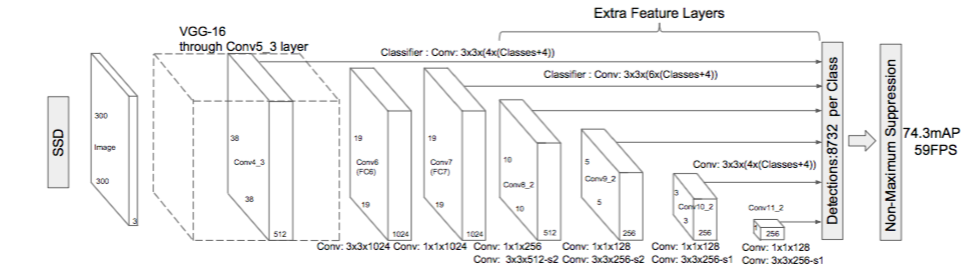
\includegraphics[width=1.0\linewidth]{ssd_architecture}
	 \caption{Arhitektura SSD mreže}
 	 \label{fig:SSDArchitecture}
\end{figure}
Slojevi dodani na baznu mrežu dodani su s ciljem da proizvedu sljedeće značajke:
